\documentclass{beamer}

\usepackage[italian]{babel}
\usepackage[utf8]{inputenc}

\usepackage{graphicx} % Immagini fantastiche e...
\graphicspath{        % dove trovarle
  {./images/},
  %{../images/}        % Necessario se cartella chapters
}

%\usepackage{float}
%\usepackage{color}
%\usepackage{caption}
%\usepackage{subcaption}

%\usepackage{hyperref}
%\hypersetup{colorlinks=true, linkcolor=black, citecolor=black, plainpages=false, urlcolor=blue}
\usepackage{wallpaper}
%\usepackage{algpseudocode,algorithm,algorithmicx}
%\usepackage{amssymb}
%\usepackage{amsmath}
%\usepackage{lipsum} 


 
% ================================ %
%          Cose Personali          %
% ================================ %
\newcommand\E{\ensuremath{\mathbb{E}}}
\newcommand\T{\ensuremath{\mathbb{T}}}
\renewcommand\inf{\ensuremath{\infty}}



%%Information to be included in the title page:
\title{Approfondimento di Intelligenza Artificiale}
\author{Tristano Munini}
%\institute{Overleaf}
  %\LARGE{\underline{\textbf{ANNO ACCADEMICO 2019-2020}}}\\
%\logo{
\includegraphics{polloPallido}}



% ================================ %
%            Il Documento          %
% ================================ %
\begin{document}

{
  \usebackgroundtemplate{
    \centering
    
\includegraphics[width=\paperwidth]{polloPallido}
  }
  \frame{\titlepage}
}

\begin{frame}
\frametitle{Introduzione}
TODO
\end{frame}


%\section{GAM}
\begin{frame}
\frametitle{template}

\begin{figure}[ht]
  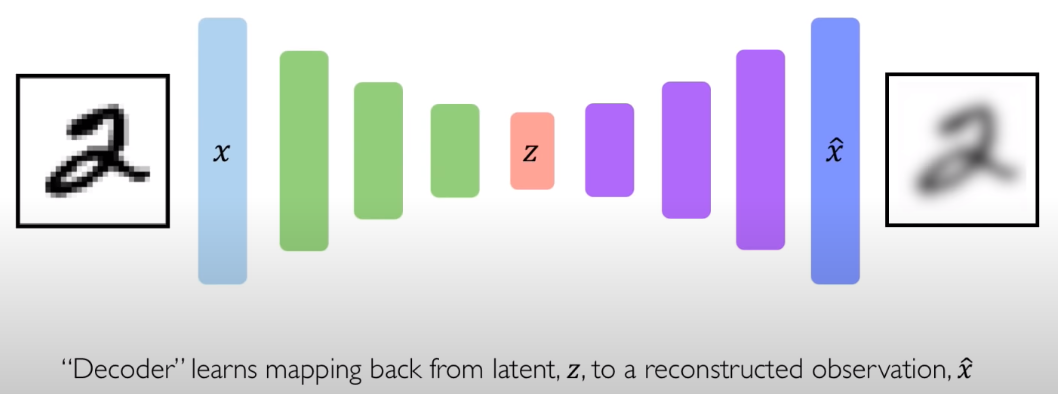
\includegraphics[width=\textwidth]{AE.png}
\end{figure}

\end{frame}

\begin{frame}
\frametitle{template}
\begin{figure}[ht]
  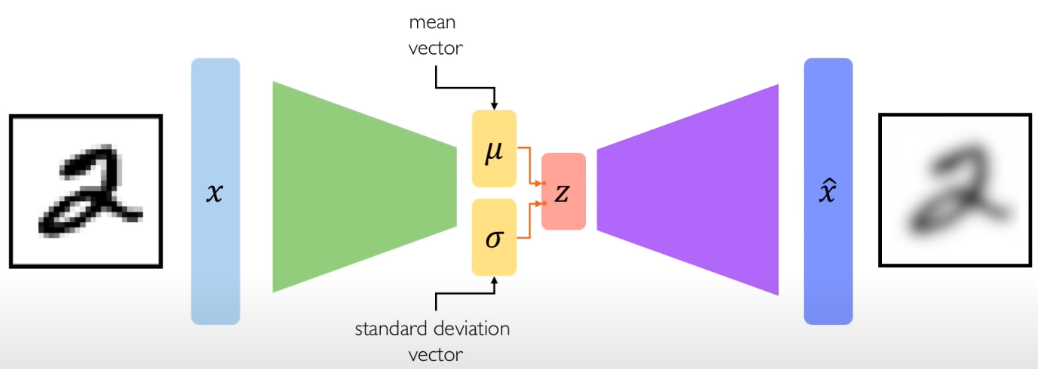
\includegraphics[width=\textwidth]{VAE.png}
\end{figure}
\end{frame}

\begin{frame}
\frametitle{template}
\begin{figure}[ht]
  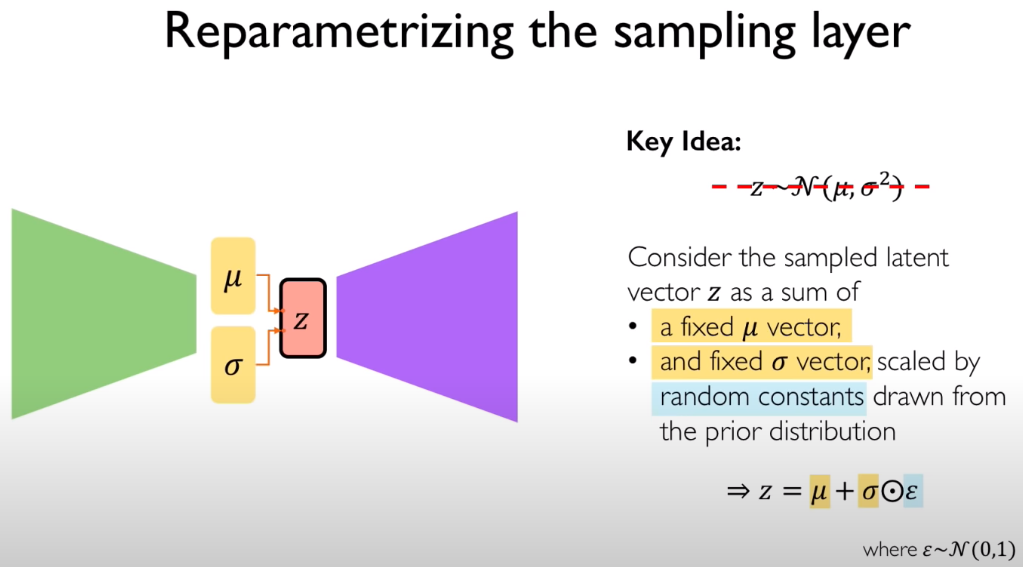
\includegraphics[width=\textwidth]{VAE_reparam_trick.png}
\end{figure}
\end{frame}

\begin{frame}
\frametitle{template}
\begin{figure}[ht]
  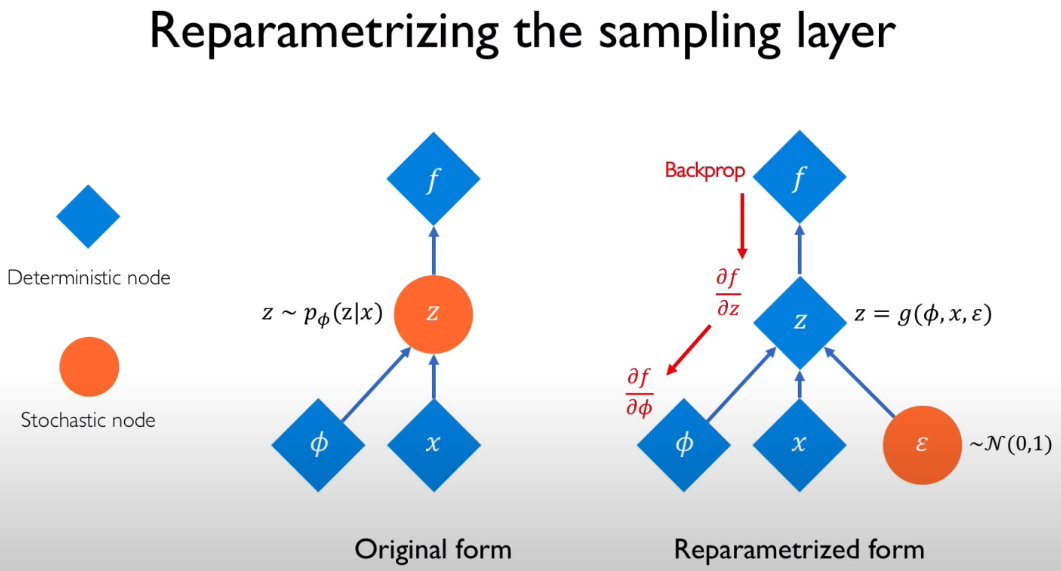
\includegraphics[width=\textwidth]{VAE_reparam_trick_backprop.png}
\end{figure}
\end{frame}


\begin{frame}
\frametitle{template}
\begin{figure}[ht]
  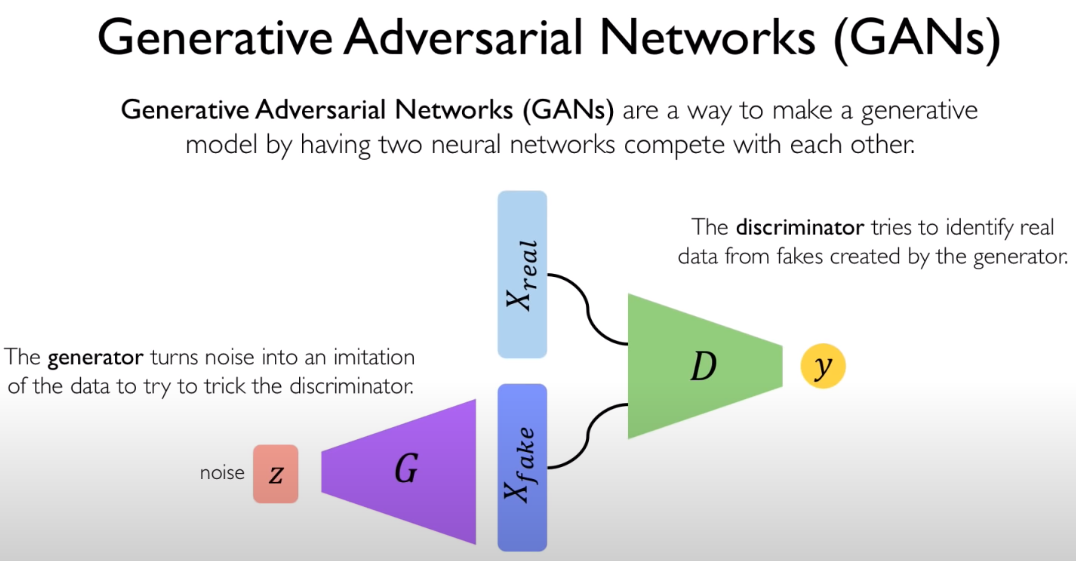
\includegraphics[width=\textwidth]{GAN.png}
\end{figure}
\end{frame}

\begin{frame}
\frametitle{template}
\begin{figure}[ht]
  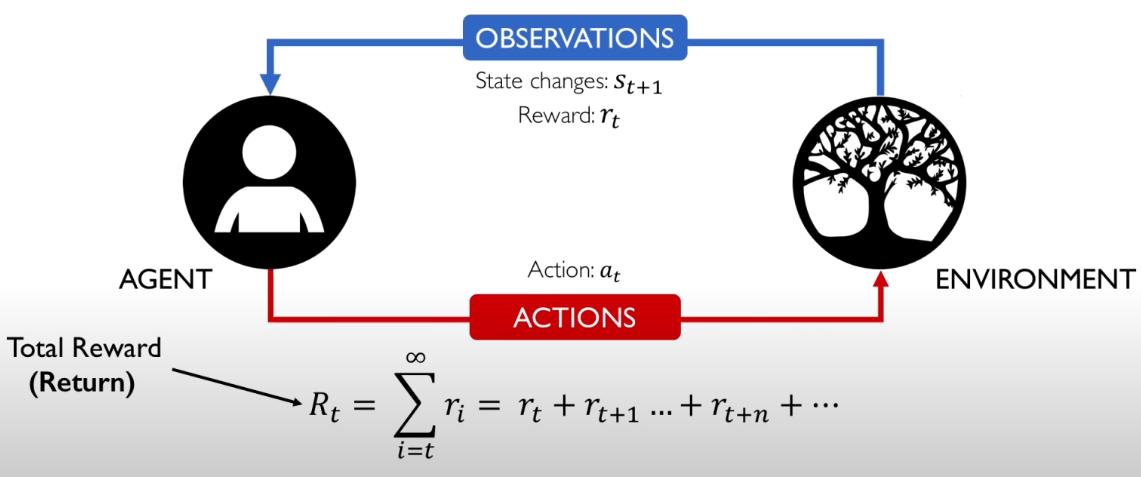
\includegraphics[width=\textwidth]{RL_key_concept.png}
  
\includegraphics[width=\textwidth]{Discounted_Total_Reward.png}
\end{figure}
\end{frame}

\begin{frame}
\frametitle{template}
\begin{figure}[ht]
  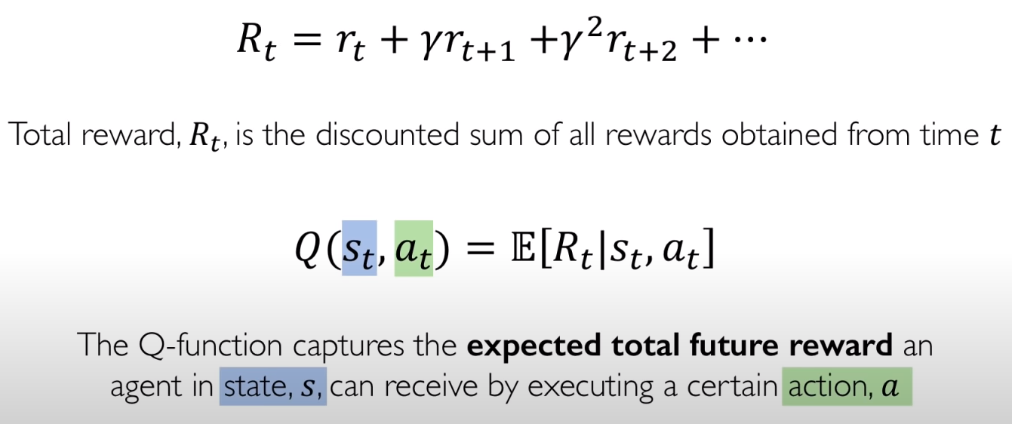
\includegraphics[width=\textwidth]{Q-Function.png}
  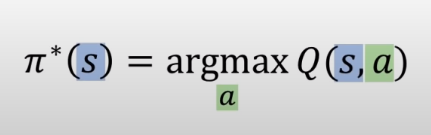
\includegraphics[width=.5\textwidth]{Policy_Fun.png}
\end{figure}
\end{frame}


%\begin{frame}
%\frametitle{template}
%\begin{figure}[ht]
%  
\includegraphics[width=\textwidth]{Discounted_Total_Reward.png}
%  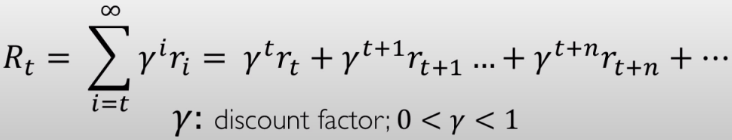
\includegraphics[width=\textwidth]{Discounted_Total_Reward_Formula.png}
%\end{figure}
%\end{frame}

\begin{frame}
\frametitle{template}
\begin{figure}[ht]
  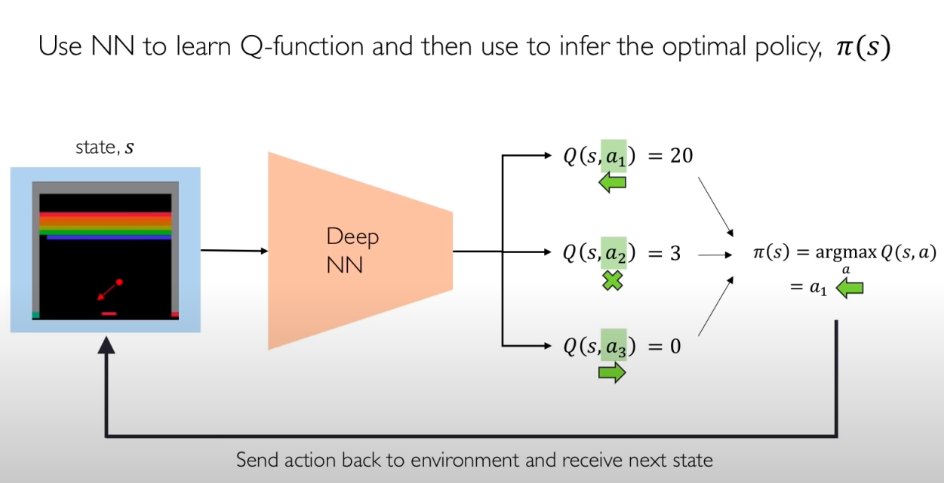
\includegraphics[width=\textwidth]{QNN.png}
\end{figure}
\end{frame}

\begin{frame}
\frametitle{template}
\begin{figure}[ht]
  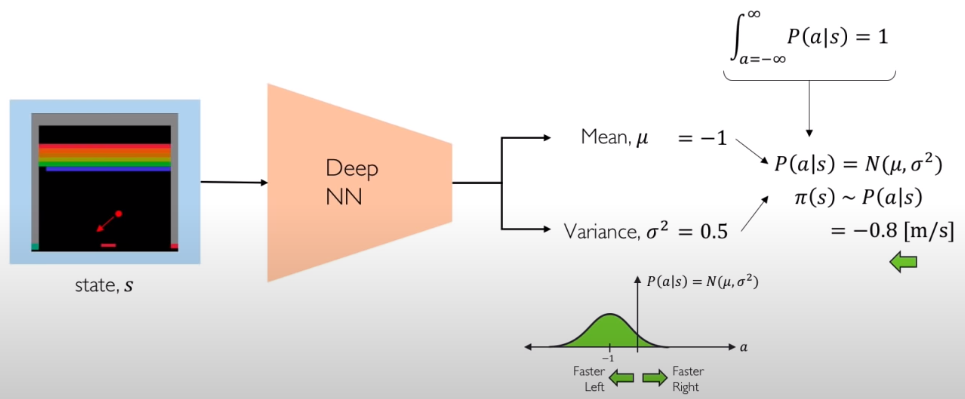
\includegraphics[width=\textwidth]{Pol_Grad.png}
\end{figure}
\end{frame}


\begin{frame}
\frametitle{template}
\begin{figure}[ht]
  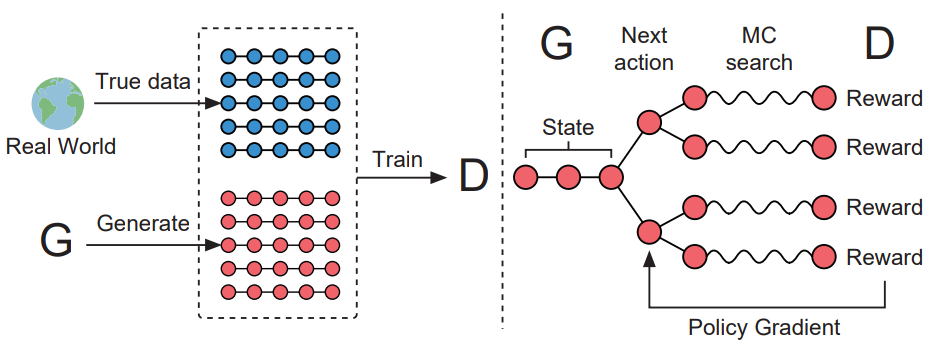
\includegraphics[width=\textwidth]{SeqGAN_Idea.png}
  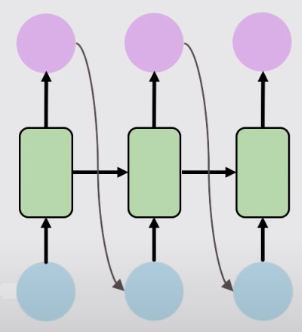
\includegraphics[width=.2\textwidth]{RNN.png}
\end{figure}
\end{frame}

%\begin{frame}
%\frametitle{template}
%\begin{figure}[ht]
%  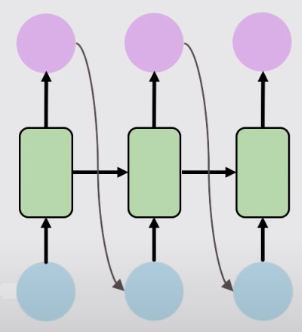
\includegraphics[width=\textwidth]{RNN.png}
%\end{figure}
%\end{frame}

\begin{frame}
\frametitle{template}
\begin{figure}[ht]
  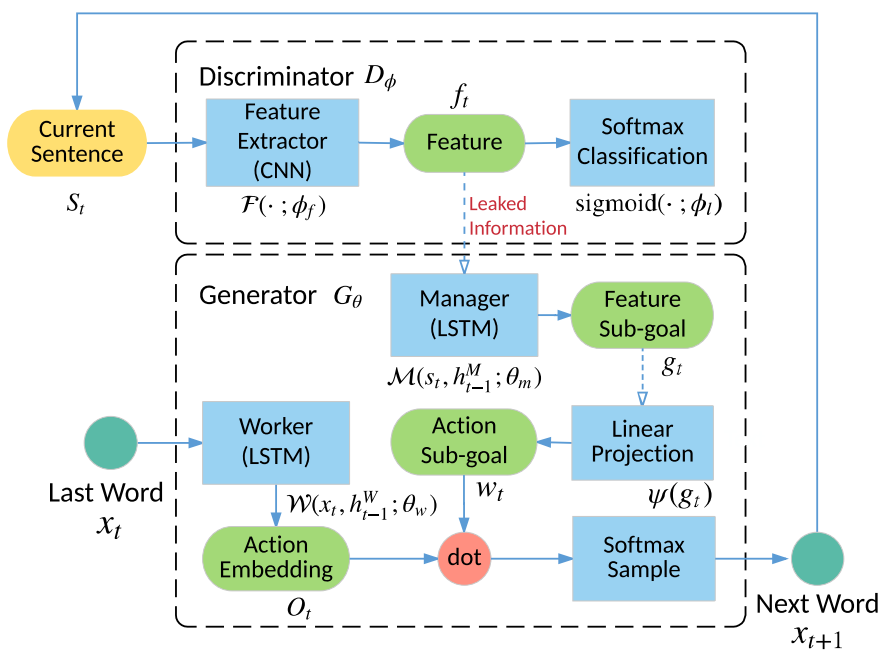
\includegraphics[width=\textwidth]{LeakGAN_Arch.png}
\end{figure}
\end{frame}

\begin{frame}
\frametitle{template}
\begin{figure}[ht]
  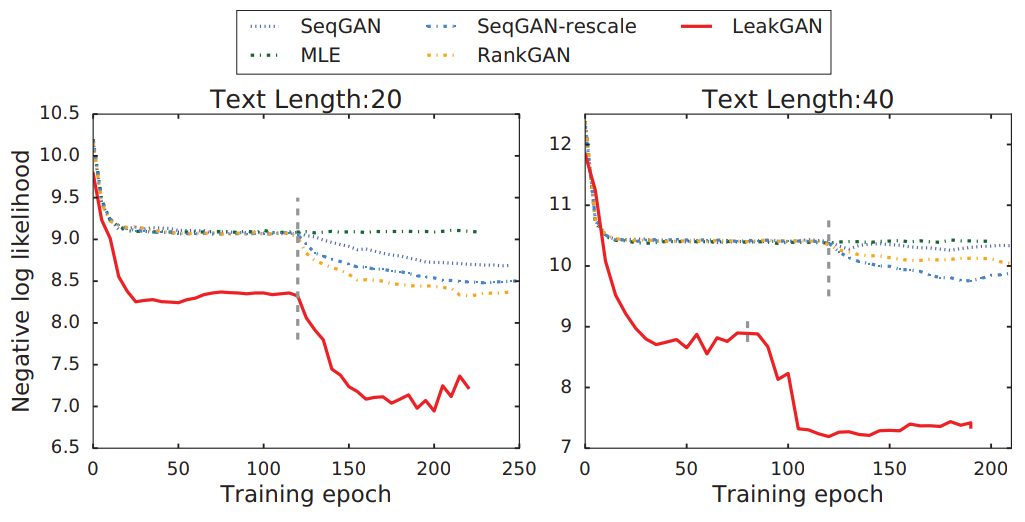
\includegraphics[width=\textwidth]{LeakGAN_vs_SeqGAN.png}
\end{figure}
\end{frame}

% AE.png
% 
% VAE.png
% VAE_reparam_trick_backprop.png
% VAE_reparam_trick.png
% 
% GAN.png
% 
% RL_key_concept.png
% Q-Function.png
% 
% Discounted_Total_Reward.png
% Discounted_Total_Reward_Formula.png
% QNN.png
% 
% Policy_Fun.png
% Pol_Grad.png
% 
% SeqGAN_Idea.png
% RNN.png
% 
% LeakGAN_Arch.png
% LeakGAN_vs_SeqGAN.png






\end{document}
